\documentclass[addpoints]{exam}
\usepackage{cmbright}
\usepackage{amsmath}
\usepackage{amssymb}
\usepackage{graphicx}
\usepackage{cite}
\usepackage[version=4]{mhchem}
\usepackage{hyperref}
\usepackage{mhchem}
\setlength\fillinlinelength{2em}

\header{CHE 525: math for CBEE's}{hw \#1: linear systems}{fall 2026}

\begin{document}

\begin{questions}

\section*{readings}

\question this course concerns mathematical tools to solve problems in engineering. an important component of the course is learning to frame a problem and make appropriate abstractions and approximations to tackle the problem. with that in mind, please read the short essays ``a systematic approach to modeling'' by chemical engineer James Riggs \cite{riggs} and ``why model?'' \cite{whymodel} by epidemiologist Joshua Epstein. the PDFs are posted on Canvas. 
\begin{parts}
	\part provide a critique of the essay of James Riggs.
	\part provide a critique of the essay of Joshua Epstein.
\end{parts}

\section*{word problems}
for each problem, be sure to sketch a picture!

\question for making white wine, freshly-picked grape clusters are de-stemmed continuously via a de-stemming machine. \emph{de-stemming} grape clusters refers to the process of separating the berries from the stems. suppose 100\,kg/hr grape clusters are fed continuously into a grape de-stemming machine. write a system of two equations for the outlet flow rate of stems and of berries via (i) an overall mass balance and (ii) using the data that the grape clusters are 7\% stems by weight \cite{grapes}. write the equations in matrix form. find the solution via Gaussian elimination. to see the row picture, draw the two equations as lines (ideally, in Python or Julia) and ensure the intersection corresponds with your solution.
\newline \textit{solution}: 7 kg/hr stems, 93 kg/hr berries.

\question a cooling crystalizer is used to form \ce{KNO3} crystals from a solution of dissolved salt in water at 100\,$^\circ$C. when 100\,kg of solution is fed to the crystallizer, which operates at 30\,$^\circ$C, 25\,kg of solid KNO$_3$ is extracted. by how many degrees Celsius is the inlet stream superheated? use the solubility data on \href{https://en.wikipedia.org/wiki/Solubility_table}{Wikipedia} (interpolate.)

\newline \textit{solution}: see \href{https://www.youtube.com/watch?v=2O4OfhqNbcs}{LearnChemE video}.

\question a pipeline network for transporting water operates at steady state. there are four nodes that cannot accumulate water. find the general solution for the network flows. what is the constraint on the flow out of $x_5$ to keep the flows in the directions shown?

\begin{figure}[htbp]
\begin{center}
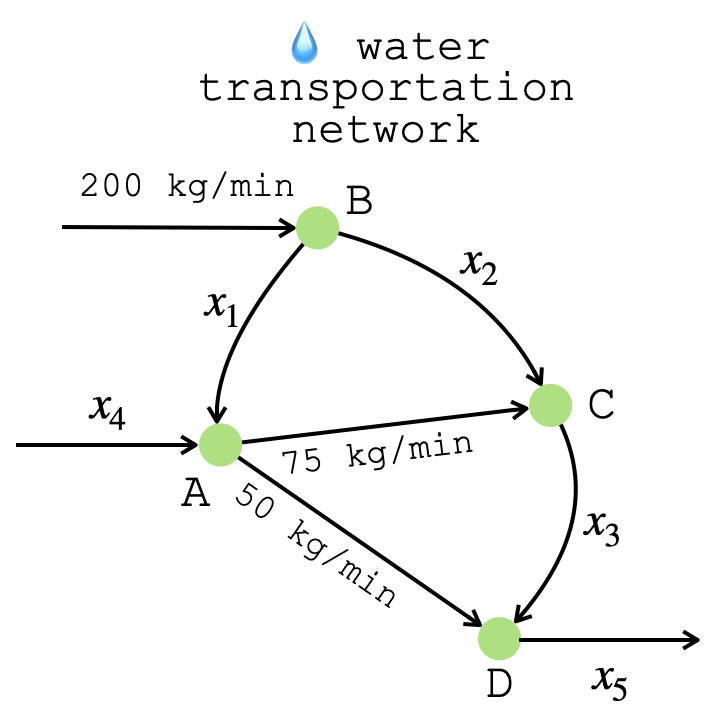
\includegraphics[width=0.4\textwidth]{transportation_network.png}
\end{center}
\end{figure}


\textit{solution}: see \href{https://webspace.ship.edu/jehamb/ela/lecture14.html}{James Hamblin's lecture 14}.

\question write a system of linear equations in matrix form to systematically balance the chemical equation describing the combustion of ethanol:

$x_1$\ce{C2H5OH} + $x_2$\ce{O2} \ce{->} $x_3$\ce{CO2} + $x_4$\ce{H2O}

use Gaussian elimination to solve the linear system.

\textit{solution}: see \href{https://allendowney.github.io/ThinkLinearAlgebra/nullspace.html#stoichiometry}{Think Linear Algebra}.


\end{questions}

\begin{thebibliography}{9}

\bibitem{riggs}
Riggs JB. A systematic approach to modeling. Chemical Engineering Education. 1988 22(1): 26-9.

\bibitem{whymodel} 
Epstein JM. Why model?. Journal of artificial societies and social simulation. 2008 11(4): 12.

\bibitem{grapes}
Blackford M, Comby M, Zeng L, Dienes-Nagy A, Bourdin G, Lorenzini F, Bach B. A review on stems composition and their impact on wine quality. Molecules. 2021 26(5) :1240.





\end{thebibliography}

\end{document}
